\documentclass[11pt]{beamer}

\usepackage{array}    % <-- For defining new column types
\usepackage{booktabs}
\usepackage{hyperref}
\usepackage{makecell} % <-- For multi-line cells
\usepackage[default]{opensans} 
\usepackage{pgffor}
\usepackage{pdfpages}
\usepackage{palatino}  
\usepackage{tcolorbox} 
\usepackage{textcomp}
\usepackage{ulem}
\usepackage{xcolor} 
\usepackage{tcolorbox} 
\usepackage{tikz}
\usepackage{tabularx}



\usetikzlibrary{arrows.meta} 
\usetikzlibrary{decorations.pathreplacing} 
\usetikzlibrary{decorations.pathmorphing}  
\usetikzlibrary{decorations.markings}     
\usetikzlibrary{decorations.text}      

\usepackage{listings}
\lstset{
  basicstyle=\ttfamily\small,
  columns=fullflexible,
  breaklines=true,
  frame=single,
  showstringspaces=false,
  showspaces=false,
  keepspaces=true,
  tabsize=4
}


\newtcbox{\highlighttexttt}{nobeforeafter, colframe=white, colback=lightgray!30, boxrule=0pt, arc=2pt, boxsep=0pt, left=1pt, right=1pt, top=1pt, bottom=1pt}
\newcommand{\hl}[1]{\colorbox{lightgray!30}{\texttt{#1}}}
\newcommand{\blink}[2]{\href{#1}{\textcolor{blue}{\underline{#2}}}}
\newcommand{\try}[1]{Have A Try: \blink{https://github.com/FSU-COP4610-F25/in-class-code}{#1}}

\usetheme{Madrid}
\usefonttheme{default} 

\useinnertheme{circles}

\setbeamertemplate{footline}{
    \leavevmode%
    \hbox{%
        \begin{beamercolorbox}[wd=0.92\paperwidth,ht=2.5ex,dp=1ex,left]{section in head/foot}
            \hspace{0.5em}
            \insertsectionnavigationhorizontal{0.9\paperwidth}{}{}
        \end{beamercolorbox}%
        \begin{beamercolorbox}[wd=0.08\paperwidth,ht=2.5ex,dp=1ex,right]{section in head/foot}
            \insertframenumber{} / \inserttotalframenumber
            \hspace{0.2em}
        \end{beamercolorbox}%
    }%
    \vskip0pt%
}


\setbeamersize{text margin left=1em, text margin right=1em}

\setbeamertemplate{frametitle}{
    \vspace{-0.5em} 
    \begin{beamercolorbox}[wd=\paperwidth,ht=2.5ex,dp=0.75ex,left]{frametitle} 
        \usebeamerfont{frametitle}\hspace{0.72em}\insertframetitle
    \end{beamercolorbox}
    \vspace{-0.5em} 
}


\newcommand{\FSUOSMeta}{%
  \author[Xin Liu]{\small Xin Liu}%
  \institute[FSU]{\small Florida State University\\[2pt]
    \href{mailto:xliu15@fsu.edu}{xliu15@fsu.edu}}%
  \date[\today]{\small CIS 4930/5930 Future Edge Networks\\[2pt]
    {\footnotesize\href{https://xinliulab.github.io/FSU-CIS4930-CIS5930-Future-Edge-Networks/}
         {\mbox{xinliulab.github.io/FSU-CIS4930-CIS5930-Future-Edge-Networks}}}}%
}

%!TEX root = ./main.tex

\usetikzlibrary{positioning,fit,backgrounds}

\definecolor{ranblue}{RGB}{46,91,186}
\definecolor{coreorange}{RGB}{222,122,36}
\definecolor{ranpurple}{RGB}{109,53,151}
\definecolor{softgreen}{RGB}{73,139,74}
\definecolor{softgray}{RGB}{92,98,105}

\newcommand{\source}[2]{%
  \par\vspace{0.25em}%
  {\tiny\textcolor{gray}{\href{#1}{\underline{#2}}}\par}%
}

% Inline expansion of an acronym at first use: SMS \expand{Short Message Service}
\newcommand{\expand}[1]{\textcolor{softgray}{(#1)}}

% Small gray glossary line, for slides with several acronyms at once.
\newcommand{\glossline}[1]{%
  \par\vspace{0.4em}%
  {\scriptsize\color{softgray}\raggedright#1\par}%
}

\newcommand{\plainterm}[2]{%
  \textbf{#1}\hspace{0.25em}{\small\textcolor{softgray}{#2}}%
}

\newcommand{\ask}[1]{%
  \begin{tcolorbox}[colback=blue!4,colframe=ranblue,boxrule=0.7pt,arc=2pt,
    left=5pt,right=5pt,top=4pt,bottom=4pt]
    \centering\large #1
  \end{tcolorbox}%
}

% Font is deliberately \normalsize, not \large: at \large a one-sentence takeaway
% wraps to two lines and the box grows into whatever is below it.
\newcommand{\takeaway}[1]{%
  \begin{tcolorbox}[colback=orange!7,colframe=coreorange,boxrule=0.7pt,arc=2pt,
    left=5pt,right=5pt,top=4pt,bottom=4pt]
    \centering\normalsize #1
  \end{tcolorbox}%
}

% Beamer overlays inside TikZ: \visible<...> breaks path parsing inside node text,
% so reveal nodes with the standard opacity idiom instead: \node[visible on=<2->] ...
\tikzset{
  invisible/.style={opacity=0,text opacity=0},
  visible on/.style={alt=#1{}{invisible}},
  alt/.code args={<#1>#2#3}{\alt<#1>{\pgfkeysalso{#2}}{\pgfkeysalso{#3}}},
}

\tikzset{
  netnode/.style={draw=ranblue,fill=blue!5,rounded corners=3pt,
    minimum width=1.9cm,minimum height=0.82cm,align=center,font=\bfseries},
  corenode/.style={draw=coreorange,fill=orange!7,rounded corners=3pt,
    minimum width=1.9cm,minimum height=0.82cm,align=center,font=\bfseries},
  oranode/.style={draw=ranpurple,fill=purple!6,rounded corners=3pt,
    minimum width=1.9cm,minimum height=0.82cm,align=center,font=\bfseries},
  flow/.style={-{Latex[length=2.4mm]},thick,draw=softgray}
}

% Full-width question/answer block: spans the whole frame, no box.
% Use below \end{columns} when the question is meant for the whole slide.
\newcommand{\qa}[2]{%
  \par\vspace{0.55em}%
  {\large\raggedright
    \noindent\hangindent=1.25em\hangafter=1
    \textcolor{ranblue}{\textbf{Q:}}\hspace{0.35em}\textbf{#1}\par
    \vspace{0.35em}
    \noindent\hangindent=1.25em\hangafter=1
    \textcolor{coreorange}{\textbf{A:}}\hspace{0.35em}#2\par}%
}

% Repeating template for "this box is gone in the next diagram" frames.
% The deck's spine: a term never vanishes between two architecture diagrams
% without a frame explaining the pressure that removed it.
% #1 what it did, #2 what broke, #3 what replaced it
\newcommand{\gonebox}[3]{%
  \vspace{0.5em}%
  \begin{columns}[T,onlytextwidth]
    \column{0.30\textwidth}
      {\small\textbf{\textcolor{softgray}{What it did}}\par}
      \vspace{0.4em}
      {\small #1\par}
    \column{0.34\textwidth}
      {\small\textbf{\textcolor{coreorange}{What broke}}\par}
      \vspace{0.4em}
      {\small #2\par}
    \column{0.30\textwidth}
      {\small\textbf{\textcolor{softgreen}{What replaced it}}\par}
      \vspace{0.4em}
      {\small #3\par}
  \end{columns}%
}

%!TEX root = ./main.tex

% Styles added for this deck; ran_macros.tex stays identical to the Wi-Fi History copy.

% Navigation symbols sit on top of the source lines at the bottom right.
\setbeamertemplate{navigation symbols}{}

\tikzset{
  % Cloud / data-center side: gray, "not ours to design".
  chnode/.style={draw=softgray,fill=gray!10,rounded corners=3pt,
    minimum width=1.7cm,minimum height=0.82cm,align=center,font=\bfseries},
  % Memory / storage blocks: green.
  kbnode/.style={draw=softgreen,fill=green!7,rounded corners=3pt,
    minimum width=1.9cm,minimum height=0.82cm,align=center,font=\bfseries},
  % Learned (neural) blocks: purple, so "trained" is visible at a glance.
  nnnode/.style={draw=ranpurple,fill=purple!6,rounded corners=3pt,
    minimum width=1.9cm,minimum height=0.82cm,align=center,font=\bfseries},
  % Plain content boxes (prompt, token, answer).
  endnode/.style={draw=softgray,fill=gray!6,rounded corners=3pt,
    minimum width=1.7cm,minimum height=1.0cm,align=center,font=\small\bfseries},
  lbl/.style={font=\scriptsize,text=softgray,align=center},
  iface/.style={font=\scriptsize\bfseries,text=coreorange},
}

% Step-by-step reveal for the colored boxes (ghost copies keep the layout stable).
\newcommand{\takeawayghost}[1]{%
  \begin{tcolorbox}[colback=orange!7,colframe=coreorange,boxrule=0.7pt,arc=2pt,
    left=5pt,right=5pt,top=4pt,bottom=4pt,
    opacityback=0,opacityframe=0,opacitytext=0]
    \centering\normalsize #1
  \end{tcolorbox}%
}
\newcommand{\askghost}[1]{%
  \begin{tcolorbox}[colback=blue!4,colframe=ranblue,boxrule=0.7pt,arc=2pt,
    left=5pt,right=5pt,top=4pt,bottom=4pt,
    opacityback=0,opacityframe=0,opacitytext=0]
    \centering\large #1
  \end{tcolorbox}%
}
\newcommand{\takeawayat}[2]{\alt<#1>{\takeaway{#2}}{\takeawayghost{#2}}}
\newcommand{\askat}[2]{\alt<#1>{\ask{#2}}{\askghost{#2}}}

% Citation line in the same style as \source, for references with no stable open URL.
\newcommand{\plainsource}[1]{%
  \par\vspace{0.25em}%
  {\tiny\textcolor{gray}{#1}\par}%
}

% A memory bar: \membar{x}{y}{width-cm}{fill-cm}{label}. Used on budget frames.
\newcommand{\membar}[5]{%
  \draw[softgray] (#1,#2) rectangle ++(#3,0.42);
  \fill[ranblue!60] (#1,#2) rectangle ++(#4,0.42);
  \node[lbl,anchor=west] at (#1+#3+0.12,#2+0.21) {#5};%
}


\title[Edge AI Systems]{Class 20: Edge AI Systems}
\subtitle{Where Should the Model Run?}

\FSUOSMeta

\begin{document}

\begin{frame}[plain]
  \titlepage
\end{frame}

\addtocounter{framenumber}{-1}

% TALK BUDGET: 50:00 = 3000 s over 34 content frames. Running example: one question
% you ask your phone ("summarize my doctor's voicemail"), answered either by the
% phone's own model or by a model in the cloud.
%   01 Intro                          0:00--3:00   2 frames  180 s
%   02 Why on-device                  3:00--8:00   3 frames  300 s
%   03 The device's budget            8:00--16:00  5 frames  480 s
%   04 Quantization                   16:00--24:00 5 frames  480 s
%   05 Mixture of Experts             24:00--33:00 5 frames  540 s
%   06 KV cache                       33:00--39:00 4 frames  360 s
%   07 Split & collaborative          39:00--45:00 4 frames  360 s
%   08 Model routing                  45:00--48:00 3 frames  180 s
%   09 Wrap-up                        48:00--50:00 3 frames  120 s
% Flex frames if running late: "And the battery" (03) compresses to 30 s; the
% speculative-decoding frame (07) can be stated in one sentence over its picture.
% Style: one idea per frame, few words; numbers rounded; anything longer is revealed
% step by step. Technical detail and sources live in each frame's "Teaching note".
%!TEX root = ./main.tex

\section[Intro]{Introduction}

% SECTION TIMING: 0:00--3:00 (2 frames): 110 + 70 s.

% Teaching note (110 s): open with the question, not the answer. You ask your phone
% to summarize a voicemail from your doctor. Two things could happen: the phone's own
% small model answers, or the audio goes to a data center and a frontier model
% answers. Take guesses on which one actually happens (answer: both exist in shipping
% products -- Apple routes between an on-device model and its cloud; Pixel runs
% Gemini Nano locally for summaries). Don't resolve the question; the lecture is the
% resolution. Point at each arrow while asking what it costs: the left arrow costs
% RAM, compute, and battery; the right arrow costs latency, privacy, and someone's
% GPU bill.
\begin{frame}{One question, two places to answer it}
  \vspace{0.8em}
  \centering
  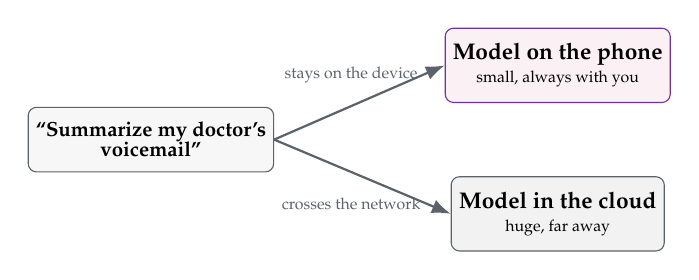
\begin{tikzpicture}[scale=0.82,transform shape]
    \node[endnode,minimum width=3.6cm] (q) at (0,0)
      {``Summarize my doctor's\\[-2pt]voicemail''};
    \node[nnnode,minimum width=3.3cm,minimum height=1.15cm] (dev) at (6.3,1.15)
      {Model on the phone\\[-2pt]{\scriptsize\mdseries small, always with you}};
    \node[chnode,minimum width=3.3cm,minimum height=1.15cm] (cloud) at (6.3,-1.15)
      {Model in the cloud\\[-2pt]{\scriptsize\mdseries huge, far away}};
    \draw[flow] (q.east) -- (dev.west);
    \draw[flow] (q.east) -- (cloud.west);
    \node[lbl] at (3.1,1.0) {stays on the device};
    \node[lbl] at (3.1,-1.0) {crosses the network};
  \end{tikzpicture}

  \vspace{0.7em}
  \askat{2-}{Where \emph{should} the model run?}

  \vspace{0.6em}
  \uncover<3->{\raggedright
    Both answers ship today: your phone has a model in it, and a data center
    has a bigger one. The interesting question is \textbf{which work goes where
    --- and why}.\par}
\end{frame}

% Teaching note (70 s): the roadmap. Read the budget line first: everything after it
% is a response to that budget. Announce the handoff: after the lecture, Lex presents
% MobileMoE (15 min + 5 min Q&A), which picks up exactly at our MoE stop. Mention
% Wednesday 11/4 continues with D2MoE (experts that do NOT fit in memory) and that
% the final project is released 11/4; HW4 is due 11/4 too.
\begin{frame}{Today's route}
  \vspace{0.5em}
  \raggedright
  \begin{enumerate}\itemsep5pt
    \item Why run AI on the device at all?
    \item The device's \textbf{budget}: memory, bandwidth, energy
    \item \textbf{Quantization} --- fewer bits per weight
    \item \textbf{Mixture of Experts} --- don't touch every weight
    \item The \textbf{KV cache} --- the memory that grows as you chat
    \item \textbf{Split} and \textbf{collaborative} inference --- cut the model in two
    \item \textbf{Model routing} --- send the hard questions away
  \end{enumerate}

  \vspace{0.7em}
  \takeawayat{2-}{One budget, five responses to it.}

  \vspace{0.5em}
  \uncover<2->{{\small After the lecture: \textbf{Lex} presents \textbf{MobileMoE}
    (stop 4, on real phones). Wednesday: \textbf{D2MoE} --- experts that
    don't fit.}\par}
\end{frame}

%!TEX root = ./main.tex

\section[Why on-device]{Why On-Device AI}

% SECTION TIMING: 3:00--8:00 (3 frames): 110 + 90 + 100 s.

% Teaching note (110 s): four reasons, one line each, revealed in order. Latency:
% recall the latency lectures -- Zhuge and SAGE fought for milliseconds across the
% network; not crossing the network at all wins by default, and a round trip to the
% cloud is tens-to-hundreds of ms before the model even starts. Privacy: the
% voicemail example -- health data; on-device means the raw data never leaves (echo
% of semantic communication: the best transmission is the one you don't make).
% Availability: airplane, basement, disaster area, or just the provider having an
% outage. Cost: every cloud query runs on a GPU someone pays for; at a billion users,
% "free" assistant queries are a real bill -- pushing work to the user's own silicon
% is the provider's favorite cost cut. None of these require the on-device model to
% be the BEST model; they require it to be good enough for the easy majority.
\begin{frame}{Four reasons to stay on the device}
  \vspace{0.6em}
  \raggedright
  \begin{description}[<+->][Availability]\itemsep7pt
    \item[Latency] no network round trip --- the answer starts now, not
      100\,ms from now
    \item[Privacy] the voicemail never leaves your phone
    \item[Availability] works on a plane, in a basement, in an outage
    \item[Cost] a billion users $\times$ free queries = someone's GPU bill;
      your phone's silicon is already paid for
  \end{description}

  \vspace{0.8em}
  \takeawayat{5-}{On-device doesn't need to beat the cloud model ---\\
    it needs to be \textbf{good enough} for the easy majority.}
\end{frame}

% Teaching note (90 s): make it concrete -- students use on-device AI daily without
% naming it: keyboard next-word prediction and autocorrect; the camera pipeline
% (night mode, portrait segmentation) runs on the NPU; "Hey Siri" / "Hey Google"
% wake-word models listen locally precisely because streaming your microphone to a
% server all day would be unacceptable; watches classify heart rhythm on the wrist;
% live translate and live captions work offline. The new part (since ~2024) is
% full LLMs on phones: Apple's on-device foundation model is on the order of 3B
% parameters, with heavier requests routed to Private Cloud Compute; Pixel ships
% Gemini Nano for summaries and smart replies. So the lecture's question is not
% hypothetical: it is a deployed architecture.
\begin{frame}{You already run models all day}
  \vspace{0.5em}
  \raggedright
  \begin{itemize}\itemsep5pt
    \item Keyboard: next-word prediction, autocorrect
    \item Camera: night mode, portrait segmentation --- on the NPU
      \expand{neural processing unit}
    \item ``Hey Siri'' / ``Hey Google'': the wake word is detected
      \textbf{locally} --- nobody streams your mic to a server all day
    \item Watch: heart-rhythm classification on the wrist
    \item Live translate, live captions: work in airplane mode
  \end{itemize}

  \vspace{0.6em}
  \uncover<2->{\raggedright New since $\sim$2024: \textbf{full LLMs} ---
    Apple runs a $\sim$3B-parameter model on the phone and routes heavy requests
    to its cloud; Pixel ships \textbf{Gemini Nano} for summaries.\par}
  \plainsource{Apple, ``Apple Intelligence Foundation Language Models,'' 2024;
    Google, Gemini Nano on Pixel, 2023--2026.}
\end{frame}

% Teaching note (100 s): steelman the cloud before the budget section, so the
% lecture doesn't read as on-device advocacy. (1) The best model simply doesn't fit:
% frontier MoE models are hundreds of GB to TB of weights. (2) Batching: a data
% center serves thousands of users per GPU, so the hardware is used efficiently;
% your NPU serves one user and idles the rest of the day. (3) One copy to update,
% measure, and guard. Then flip it: the real design isn't a side to pick but a
% partition -- which brings us to what the device can actually afford. The last
% line hands off to the budget section.
\begin{frame}{The cloud's counterargument}
  \vspace{0.6em}
  \raggedright
  \begin{itemize}[<+->]\itemsep7pt
    \item The best model \textbf{doesn't fit}: frontier models are hundreds of
      GB of weights
    \item A data-center GPU is \textbf{shared}: thousands of users batch on one
      card; your NPU serves one user, then idles
    \item One copy in the cloud: always updated, measured, guarded
  \end{itemize}

  \vspace{0.9em}
  \takeawayat{4-}{Not ``device \emph{vs.} cloud'' --- a \textbf{partition}:
    which part of the work runs where?}

  \vspace{0.4em}
  \uncover<4->{{\small To partition well, we first need the device's budget.}\par}
\end{frame}

%!TEX root = ./main.tex

\section[Budget]{The Device's Budget}

% SECTION TIMING: 8:00--16:00 (5 frames): 100 + 110 + 120 + 90 + 60 s.
% Flex: "And the battery" compresses to 30 s (read the takeaway, skip the joule talk).

% Teaching note (100 s): establish the one mechanical fact the whole lecture rests
% on. An LLM generates text one token at a time; to produce ONE token, the model
% multiplies through essentially ALL of its weights. So two numbers decide
% everything: how many bytes the weights occupy (do they fit?), and how many bytes
% per second the memory can deliver (how fast can we read them, once per token?).
% Walk the picture left to right: prompt in, one token out, and the fat arrow is
% the weights being read -- again for the next token, and again. Computing is not
% the fat arrow; reading is.
\begin{frame}{What one token costs}
  \vspace{0.8em}
  \centering
  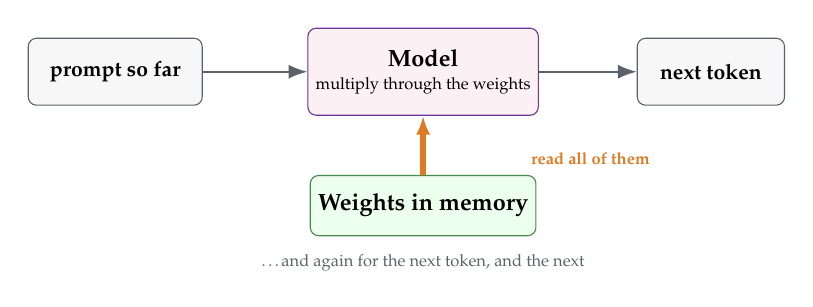
\begin{tikzpicture}[scale=0.85,transform shape]
    \node[endnode,minimum width=2.6cm] (in) at (0,0) {prompt so far};
    \node[nnnode,minimum width=3.2cm,minimum height=1.3cm] (m) at (4.6,0)
      {Model\\[-2pt]{\scriptsize\mdseries multiply through the weights}};
    \node[endnode,minimum width=2.2cm] (out) at (8.9,0) {next token};
    \draw[flow] (in) -- (m);
    \draw[flow] (m) -- (out);
    \node[kbnode,minimum width=3.2cm,minimum height=0.9cm,visible on=<2->]
      (w) at (4.6,-2.0) {Weights in memory};
    \draw[flow,line width=2.2pt,draw=coreorange,visible on=<2->]
      (w.north) -- (m.south);
    \node[iface,visible on=<2->] at (7.1,-1.3) {read \textbf{all} of them};
    \node[lbl,visible on=<3->] at (4.6,-2.85)
      {\ldots and again for the next token, and the next};
  \end{tikzpicture}

  \vspace{0.8em}
  \takeawayat{4-}{Two numbers rule on-device LLMs:\\
    \textbf{bytes the weights occupy} and \textbf{bytes/second the memory delivers}.}
\end{frame}

% Teaching note (110 s): the budget table. Phone: 8--12 GB RAM, shared with the OS
% and every app -- the model may claim a few GB at best; LPDDR5X delivers roughly
% 60--80 GB/s; sustained power a few watts before thermal throttling (it sits in a
% hand or pocket). Laptop: tens of GB, 100--400 GB/s (Apple M-series unified
% memory). Data-center GPU: H100 = 80 GB of HBM3 at 3.35 TB/s, ~700 W. The point of
% the table is the two orders of magnitude in bandwidth between phone and GPU --
% same math, wildly different budgets. Numbers are rounded; exact SKUs differ.
\begin{frame}{The budget, by device}
  \vspace{0.6em}
  \centering
  \begin{tabular}{@{}lccc@{}}
    \toprule
    & \textbf{Phone} & \textbf{Laptop} & \textbf{Cloud GPU (H100)}\\
    \midrule
    Memory for the model & a few GB & tens of GB & 80 GB HBM\\
    Memory bandwidth & $\sim$70 GB/s & 100--400 GB/s & 3{,}350 GB/s\\
    Sustained power & a few W & tens of W & $\sim$700 W\\
    Serving & you & you & thousands of users\\
    \bottomrule
  \end{tabular}

  \vspace{0.9em}
  \uncover<2->{\raggedright The GPU's memory is $\sim$\textbf{50$\times$ faster}
    than the phone's. Same math, a very different budget.\par}
  \plainsource{Rounded, representative figures: LPDDR5X-class phones ($\sim$2024--26);
    Apple M-series unified memory; NVIDIA H100 SXM (80 GB HBM3, 3.35 TB/s).}
\end{frame}

% Teaching note (120 s): THE arithmetic frame -- do it slowly, on the board if
% possible. A 7B-parameter model at FP16 is 7B x 2 bytes = 14 GB: does not fit in a
% phone's few GB. Pretend it did: every token must read 14 GB; at 70 GB/s that is
% at most 70/14 = 5 tokens/s -- around human reading speed, with zero margin.
% Both problems point at the same lever: shrink the bytes. Preview: at 4 bits per
% weight the same model is 3.5 GB (fits) and the ceiling becomes 70/3.5 = 20
% tokens/s. That lever is the next section. Keep the "upper bound" honest: real
% systems lose some bandwidth to the KV cache and activations, so these are
% ceilings, not predictions.
\begin{frame}{Do the math: a 7B model on a phone}
  \vspace{0.5em}
  \raggedright
  {\large\textbf{Fit?}}\par
  \vspace{0.2em}
  7B weights $\times$ 2 bytes (FP16) $=$ \textbf{14 GB}
  \hspace{0.6em}---\hspace{0.6em} the phone has \textbf{a few GB} to spare.
  \textcolor{coreorange}{\textbf{Doesn't fit.}}\par

  \vspace{0.8em}
  \uncover<2->{{\large\textbf{Fast enough, even if it fit?}}\par
    \vspace{0.2em}
    every token reads 14 GB; at 70 GB/s:
    \quad $\dfrac{70\ \text{GB/s}}{14\ \text{GB}} = $ \textbf{5 tokens/s} at best
    --- reading speed, zero margin.\par}

  \vspace{0.8em}
  \takeawayat{3-}{Both walls are made of \textbf{bytes}.\\
    Every trick today is a way to move fewer of them.}
\end{frame}

% Teaching note (90 s): one asymmetry to name now because MoE and split inference
% both exploit it. PREFILL: the prompt's tokens are all known, so the device
% processes them in parallel -- lots of arithmetic per byte read -- compute-bound.
% DECODE: tokens come out one at a time; each step reads all weights to produce one
% token -- bandwidth-bound. That is why the time-to-first-token and the
% tokens-per-second afterwards behave differently, and why some tricks help one
% phase and not the other (quantization helps decode a lot; a faster NPU helps
% prefill). Students have felt this: the pause before the first word vs. the
% streaming speed afterwards.
\begin{frame}{Two phases, two bottlenecks}
  \vspace{0.6em}
  \centering
  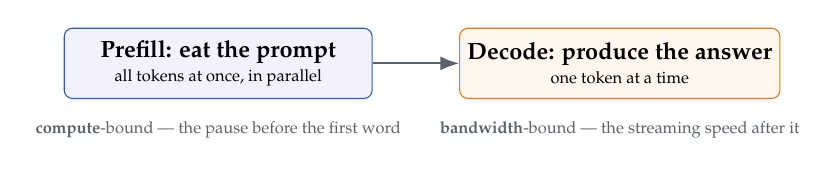
\begin{tikzpicture}[scale=0.85,transform shape]
    \node[netnode,minimum width=4.6cm,minimum height=1.05cm] (pre) at (0,0)
      {Prefill: eat the prompt\\[-2pt]{\scriptsize\mdseries all tokens at once,
        in parallel}};
    \node[corenode,minimum width=4.6cm,minimum height=1.05cm] (dec) at (6.0,0)
      {Decode: produce the answer\\[-2pt]{\scriptsize\mdseries one token
        at a time}};
    \draw[flow] (pre) -- (dec);
    \node[lbl,visible on=<2->] at (0,-1.0)
      {\textbf{compute}-bound --- the pause before the first word};
    \node[lbl,visible on=<2->] at (6.0,-1.0)
      {\textbf{bandwidth}-bound --- the streaming speed after it};
  \end{tikzpicture}

  \vspace{0.9em}
  \takeawayat{3-}{You have felt both: the \textbf{pause}, then the
    \textbf{stream}.\\ Different walls, different fixes.}
\end{frame}

% Teaching note (60 s, flex to 30 s): energy seals the argument. Moving a byte in
% from DRAM costs orders of magnitude more energy than one arithmetic operation on
% it -- so the bandwidth wall is also the battery wall; the same fix (fewer bytes)
% serves both. And a phone throttles on heat: it sits in a hand, with no fan.
% Sustained token generation at full tilt turns into a warm phone and a lower
% clock. Mention once, move on.
\begin{frame}{And the battery agrees}
  \vspace{0.8em}
  \raggedright
  \begin{itemize}\itemsep7pt
    \item Moving a byte from DRAM costs \textbf{far more energy} than computing
      with it once it has arrived
    \item No fan, held in a hand: sustained generation $\rightarrow$ heat
      $\rightarrow$ \textbf{throttling}
  \end{itemize}

  \vspace{1.0em}
  \takeawayat{2-}{The bandwidth wall and the battery wall are the
    \textbf{same wall}:\\ bytes moved. One fix serves both.}
\end{frame}

%!TEX root = ./main.tex

\section[Quantization]{Quantization}

% SECTION TIMING: 16:00--24:00 (5 frames): 90 + 100 + 110 + 110 + 70 s.

% Teaching note (90 s): the idea in one picture. A weight is just a number stored in
% bits; training uses 16-bit floats. Quantization stores each weight in 8 or 4 bits
% instead: map the range of values in a group of weights onto a small grid of
% levels, store the grid index, keep one scale factor per group to map back. The
% model is not retrained (post-training quantization); we only re-encode the
% numbers. Analogy that lands: rounding every price in a store to the nearest
% dollar -- the catalog shrinks, most totals barely change.
\begin{frame}{Trick 1: store each weight in fewer bits}
  \vspace{0.7em}
  \centering
  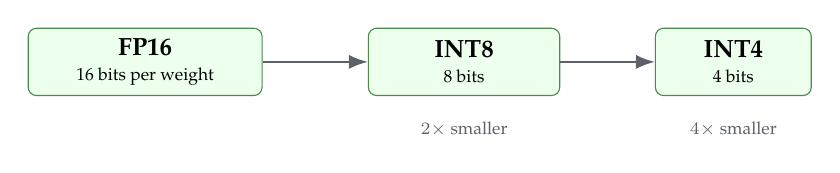
\begin{tikzpicture}[scale=0.9,transform shape]
    \node[kbnode,minimum width=3.3cm,minimum height=0.95cm] (fp) at (0,0)
      {FP16\\[-2pt]{\scriptsize\mdseries 16 bits per weight}};
    \node[kbnode,minimum width=2.7cm,minimum height=0.95cm,visible on=<2->]
      (i8) at (4.5,0) {INT8\\[-2pt]{\scriptsize\mdseries 8 bits}};
    \node[kbnode,minimum width=2.2cm,minimum height=0.95cm,visible on=<2->]
      (i4) at (8.3,0) {INT4\\[-2pt]{\scriptsize\mdseries 4 bits}};
    \draw[flow,visible on=<2->] (fp) -- (i8);
    \draw[flow,visible on=<2->] (i8) -- (i4);
    \node[lbl,visible on=<2->] at (4.5,-0.95) {$2\times$ smaller};
    \node[lbl,visible on=<2->] at (8.3,-0.95) {$4\times$ smaller};
  \end{tikzpicture}

  \vspace{0.7em}
  \uncover<3->{\raggedright Round each weight onto a coarse grid; keep one
    \textbf{scale} per group of weights to map back. No retraining ---
    just re-encoding the numbers.\par}

  \vspace{0.5em}
  \takeawayat{4-}{Like rounding every price to the nearest dollar:\\
    the catalog shrinks, most totals barely move.}
\end{frame}

% Teaching note (100 s): redo the budget math with 4 bits -- same frame layout as
% "Do the math" on purpose, so the payoff is visible. 7B x 0.5 byte = 3.5 GB: now it
% fits beside the OS. Ceiling: 70/3.5 = 20 tokens/s -- a comfortable chat. And since
% decode is bandwidth-bound, the 4x fewer bytes read per token is a real ~4x on
% streaming speed, not a paper number. This is why every on-device LLM ships
% quantized.
\begin{frame}{The same math at 4 bits}
  \vspace{0.5em}
  \raggedright
  {\large\textbf{Fit?}}\par
  \vspace{0.2em}
  7B weights $\times$ 0.5 byte (INT4) $=$ \textbf{3.5 GB}
  \hspace{0.6em}---\hspace{0.6em} \textcolor{softgreen}{\textbf{fits}} next to
  the OS.\par

  \vspace{0.8em}
  \uncover<2->{{\large\textbf{Fast enough?}}\par
    \vspace{0.2em}
    every token now reads 3.5 GB:
    \quad $\dfrac{70\ \text{GB/s}}{3.5\ \text{GB}} = $ \textbf{20 tokens/s}
    --- a comfortable chat.\par}

  \vspace{0.8em}
  \takeawayat{3-}{Decode is bandwidth-bound, so $4\times$ fewer bytes\\
    $\approx$ $4\times$ faster streaming. Not a paper number --- you feel it.}
\end{frame}

% Teaching note (110 s): why it isn't free. Draw the histogram story in words: most
% weights are small and cluster near zero; a few channels carry outliers -- values
% far outside the pack. One shared grid must stretch to cover the outliers, so the
% small weights all collapse onto a few levels and the layer's output drifts. At 8
% bits there is enough resolution to hide this; at 4 bits naive rounding visibly
% hurts: answers get vaguer, arithmetic and code break first. The sketch shows the
% quality cliff: flat from 16 to 8, bends at 4, dives below 3. The orange dot --
% "where on-device wants to live" -- is exactly on the bend; that tension motivates
% the next frame.
\begin{frame}{Why 4 bits is not free}
  \vspace{0.5em}
  \raggedright
  A few \textbf{outlier} weights stretch the grid; the many small weights
  collapse onto a few levels.\par

  \vspace{0.6em}
  \centering
  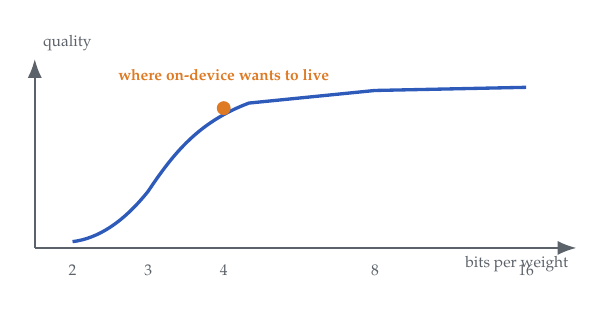
\begin{tikzpicture}[scale=0.8,transform shape]
    \draw[flow] (0,0) -- (8.6,0) node[lbl,below left] {bits per weight};
    \draw[flow] (0,0) -- (0,3.0) node[lbl,above right] {quality};
    \node[lbl] at (7.8,-0.35) {16};
    \node[lbl] at (5.4,-0.35) {8};
    \node[lbl] at (3.0,-0.35) {4};
    \node[lbl] at (1.8,-0.35) {3};
    \node[lbl] at (0.6,-0.35) {2};
    \draw[very thick,ranblue]
      (7.8,2.55) -- (5.4,2.5) -- (3.4,2.3) .. controls (2.6,2.0) and (2.2,1.5)
      .. (1.8,0.9) .. controls (1.4,0.4) and (1.0,0.15) .. (0.6,0.1);
    \fill[coreorange,visible on=<2->] (3.0,2.22) circle (0.11);
    \node[iface,visible on=<2->] at (3.0,2.75) {where on-device wants to live};
  \end{tikzpicture}

  \vspace{0.5em}
  \takeawayat{3-}{Flat from 16 to 8 bits; the cliff starts right where\\
    the phone needs to be. Naive rounding falls off it.}
\end{frame}

% Teaching note (110 s): how real quantizers stay on the ledge, at intuition level
% only -- no algorithm details. Three ideas: (1) calibrate -- run a few hundred
% sample inputs through the model and choose each group's grid to minimize the error
% that actually shows up in the layer's output, instead of rounding blindly;
% (2) protect what matters -- keep the outlier channels (~1% of weights) in higher
% precision, or scale them down before rounding so the shared grid fits the rest
% (that is AWQ's observation; GPTQ instead corrects remaining weights as it rounds);
% (3) weights are the easy half -- activations change with every input, so
% activation quantization is harder; on phones, weights-only INT4 with FP16 compute
% is the common recipe. Name-drop GPTQ/AWQ in gray for students who want to read.
\begin{frame}{How real quantizers stay on the ledge}
  \vspace{0.6em}
  \raggedright
  \begin{enumerate}[<+->]\itemsep7pt
    \item \textbf{Calibrate}: run a few hundred sample inputs; pick each grid to
      minimize the error that actually appears in the output
    \item \textbf{Protect the outliers}: keep the $\sim$1\% extreme channels in
      higher precision --- or rescale them so the shared grid fits the rest
    \item \textbf{Weights first}: activations change with every input and are
      harder --- phones mostly ship \emph{weights-only} INT4
  \end{enumerate}

  \vspace{0.7em}
  \glossline{Reading, if you want the algorithms: GPTQ (round, then correct the
    remaining weights) and AWQ (rescale the salient channels before rounding).}
  \plainsource{Frantar et al., ``GPTQ,'' ICLR 2023; Lin et al., ``AWQ,''
    MLSys 2024 (Best Paper).}
\end{frame}

% Teaching note (70 s): close the section by pointing at shipping systems: Apple's
% on-device foundation model averages about 3.7 bits per weight (mixed 2- and
% 4-bit, published in their 2024 report); Gemini Nano and the open on-device models
% students can run (llama.cpp's 4-bit GGUF files) are the same idea. The takeaway
% restates the lecture's spine: quantization shrinks every byte; the next section
% instead avoids touching most bytes at all -- hand off to MoE.
\begin{frame}{Quantization, in the wild}
  \vspace{0.7em}
  \raggedright
  \begin{itemize}\itemsep7pt
    \item Apple's on-device model: $\sim$\textbf{3.7 bits} per weight on average
      (mixed 2-/4-bit)
    \item Gemini Nano, and every 4-bit model file you can run with
      \texttt{llama.cpp}: same idea
  \end{itemize}
  \plainsource{Apple, ``Apple Intelligence Foundation Language Models,'' 2024.}

  \vspace{0.9em}
  \takeawayat{2-}{Quantization makes every byte smaller.\\
    Next trick: \textbf{don't touch most bytes at all}.}
\end{frame}

%!TEX root = ./main.tex

\section[MoE]{Mixture of Experts}

% SECTION TIMING: 24:00--33:00 (5 frames): 120 + 100 + 100 + 130 + 90 s.

% Teaching note (120 s): the structure in one picture. In a dense model, every token
% multiplies through every weight of every layer. An MoE layer replaces one big
% feed-forward block with many smaller "experts" plus a tiny router; the router
% scores the token and sends it through only the top-k experts. Walk the picture:
% the token hits the router, two experts light up, the rest stay dark -- capacity
% (total weights) grew, but compute per token stayed small. The term of art is
% "active parameters": the subset actually touched for this token.
\begin{frame}{Trick 2: many experts, use a few}
  \vspace{0.6em}
  \centering
  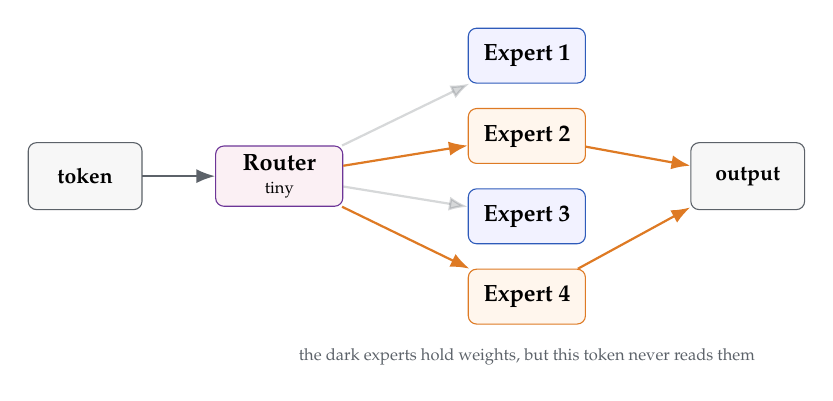
\begin{tikzpicture}[scale=0.85,transform shape]
    \node[endnode,minimum width=1.7cm] (tok) at (0,0) {token};
    \node[nnnode,minimum width=1.9cm,minimum height=0.9cm] (r) at (2.9,0)
      {Router\\[-2pt]{\scriptsize\mdseries tiny}};
    \node[netnode,minimum width=1.75cm,visible on=<2->] (e1) at (6.6,1.8)
      {Expert 1};
    \node[corenode,minimum width=1.75cm] (e2) at (6.6,0.6) {Expert 2};
    \node[netnode,minimum width=1.75cm,visible on=<2->] (e3) at (6.6,-0.6)
      {Expert 3};
    \node[corenode,minimum width=1.75cm] (e4) at (6.6,-1.8) {Expert 4};
    \node[endnode,minimum width=1.7cm] (out) at (9.9,0) {output};
    \draw[flow] (tok) -- (r);
    \draw[flow,draw=coreorange,thick] (r) -- (e2);
    \draw[flow,draw=coreorange,thick] (r) -- (e4);
    \draw[flow,draw=coreorange,thick] (e2) -- (out);
    \draw[flow,draw=coreorange,thick] (e4) -- (out);
    \draw[flow,opacity=0.25,visible on=<2->] (r) -- (e1);
    \draw[flow,opacity=0.25,visible on=<2->] (r) -- (e3);
    \node[lbl,visible on=<2->] at (6.6,-2.7)
      {the dark experts hold weights, but this token never reads them};
  \end{tikzpicture}

  \vspace{0.6em}
  \takeawayat{3-}{Total capacity grows; \textbf{active} weights per token
    stay small.\\ You store a big model but \emph{read} a small one.}
\end{frame}

% Teaching note (100 s): why the data center loves this. DeepSeek-V3: 671B total
% parameters, ~37B active per token -- the quality of a huge model at the read cost
% of a mid-size one. The course page's own line: essentially every frontier model of
% 2025 -- DeepSeek-V3, Llama 4, Qwen3, gpt-oss -- is an MoE. The data center's
% budget makes this trade easy: HBM capacity is there to hold all experts, batching
% keeps every expert busy across thousands of users, and compute per token is the
% scarce resource being saved.
\begin{frame}{Why every frontier model went MoE}
  \vspace{0.6em}
  \raggedright
  \begin{itemize}\itemsep6pt
    \item DeepSeek-V3: \textbf{671B} parameters total, $\sim$\textbf{37B active}
      per token
    \item Llama 4, Qwen3, gpt-oss: all MoE --- the 2025 frontier default
  \end{itemize}

  \vspace{0.6em}
  \uncover<2->{\raggedright The data center's trade: memory is
    \textbf{plentiful} (80 GB HBM per GPU, many GPUs), compute per token is the
    scarce thing. MoE spends memory to save compute.\par}

  \vspace{0.7em}
  \takeawayat{3-}{MoE buys capacity \textbf{with memory} instead of compute\\
    --- perfect for a data center.}
  \plainsource{DeepSeek-AI, ``DeepSeek-V3 Technical Report,'' 2024.}
\end{frame}

% Teaching note (100 s): now flip the budget. The phone has the opposite scarcity:
% memory is the thing it does not have -- idle experts still occupy RAM; and the
% router's per-token choices mean different tokens touch different experts, so
% across a sentence most experts get paged through anyway unless the design keeps
% them small. Ask the class the question before revealing: "same trick, opposite
% budget -- what should change?" Expected intuitions: fewer/smaller experts, keep a
% shared always-on expert, pick more experts per token so each can be tiny, or
% don't keep them all in RAM. All four appear in the next two frames.
\begin{frame}{A phone flips the trade}
  \vspace{0.7em}
  \raggedright
  \begin{itemize}\itemsep7pt
    \item Idle experts still \textbf{occupy RAM} --- the resource the phone
      lacks most
    \item Every weight touched is \textbf{bandwidth paid} --- and each token
      picks different experts
    \item One user, no batching --- dark experts earn nothing while they sit
  \end{itemize}

  \vspace{0.9em}
  \askat{2-}{Same trick, opposite budget:\\ what should an MoE look like
    \emph{on a phone}?}
\end{frame}

% Teaching note (130 s): set up Lex's talk without giving it away -- state the
% question MobileMoE answers and its headline shape, and leave the "how" to the
% presentation. Meta fitted an MoE scaling law on real smartphones (actual latency
% and memory measurements, not FLOP counts) and asked: at a FIXED weight-memory
% budget, what sparsity and expert granularity maximize quality and speed? Their
% answer: moderate sparsity, fine-grained experts -- 60 routed experts + 1 shared
% expert, route to the top 4. The shared expert handles what every token needs, so
% routed experts stay small and the active-bytes-per-token shrink. Result, at equal
% weight memory: 1.8--3.8x faster prefill and 2.2--3.4x faster decode than a dense
% model of the same memory. The frame intentionally shows the numbers, not the
% method -- the method is Lex's 15 minutes.
\begin{frame}{MobileMoE: the phone-shaped answer (teaser)}
  \vspace{0.6em}
  \raggedright
  Meta fitted an MoE \textbf{scaling law on real smartphones} and asked: at a
  fixed weight-memory budget, what shape wins?\par

  \vspace{0.6em}
  \uncover<2->{\begin{itemize}\itemsep5pt
    \item \textbf{60 routed experts + 1 shared}, route to \textbf{top-4} ---
      fine-grained, moderately sparse
    \item At \emph{equal weight memory} vs.\ dense:
      \textbf{1.8--3.8$\times$} faster prefill,
      \textbf{2.2--3.4$\times$} faster decode
  \end{itemize}\par}

  \vspace{0.7em}
  \takeawayat{3-}{Capacity with \emph{small active bytes per token}\\
    --- MoE reshaped for the phone's budget.}

  \vspace{0.4em}
  \uncover<3->{{\small The how --- the scaling law, the shared expert, the
    measurements --- is \textbf{Lex's talk}, right after this lecture.}\par}
  \plainsource{MobileMoE: Scaling On-Device Mixture of Experts, Meta, arXiv,
    May 2026.}
\end{frame}

% Teaching note (90 s): the loose end that Wednesday pulls. MobileMoE still assumes
% every expert fits in RAM. Suppose they don't: the natural move is a memory
% hierarchy -- hot experts in RAM, cold experts in flash, predict which experts the
% next tokens will route to and prefetch them. Flash is fast enough to stream a
% small expert if you guess early and are right most of the time; guess late or
% wrong and decode stalls. That exact problem -- which expert to keep, which to
% spill, when to prefetch -- is D2MoE on Wednesday 11/4. One sentence of preview,
% no more.
\begin{frame}{The loose end: experts that don't fit}
  \vspace{0.7em}
  \centering
  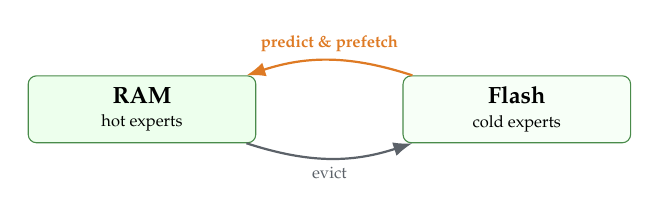
\begin{tikzpicture}[scale=0.85,transform shape]
    \node[kbnode,minimum width=3.4cm,minimum height=1.0cm] (ram) at (0,0)
      {RAM\\[-2pt]{\scriptsize\mdseries hot experts}};
    \node[kbnode,minimum width=3.4cm,minimum height=1.0cm,fill=green!3] (fl)
      at (5.6,0) {Flash\\[-2pt]{\scriptsize\mdseries cold experts}};
    \draw[flow,draw=coreorange,thick] (fl) to[bend right=18]
      node[iface,above] {predict \& prefetch} (ram);
    \draw[flow] (ram) to[bend right=18] node[lbl,below] {evict} (fl);
  \end{tikzpicture}

  \vspace{0.8em}
  \raggedright
  Guess the next experts early and right, and decode never notices.
  Guess wrong, and it stalls on flash.\par

  \vspace{0.6em}
  \takeawayat{2-}{Which experts to keep, spill, and prefetch ---\\
    that is \textbf{D2MoE}, Wednesday 11/4.}
\end{frame}

%!TEX root = ./main.tex

\section[KV cache]{The KV Cache}

% SECTION TIMING: 33:00--39:00 (4 frames): 110 + 100 + 90 + 60 s.

% Teaching note (110 s): connect to the 10/19 PyTorch lecture (attention appeared in
% the CNN/RNN/Transformer demo). To produce token N, attention compares the new
% token's query against a key and value for EVERY previous token. Recomputing all
% those keys and values from scratch each step would redo the whole prompt's work
% every token -- so every serious implementation computes each token's K and V once
% and caches them. The picture: tokens stream in, each drops a small (K,V) brick
% into a growing shelf; the new token reads the whole shelf. The cache is pure
% speed-for-memory: nothing is approximated -- yet.
\begin{frame}{Trick 3's target: the cache you didn't know you had}
  \vspace{0.6em}
  \raggedright
  Attention: the new token compares against a \textbf{key} and \textbf{value}
  for \emph{every} previous token (PyTorch lecture, 10/19).\par

  \vspace{0.6em}
  \centering
  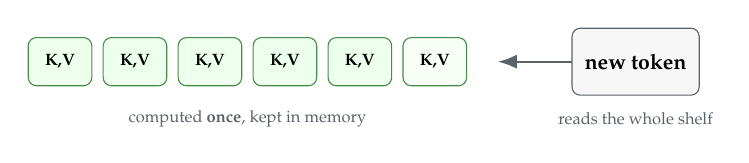
\begin{tikzpicture}[scale=0.85,transform shape]
    \foreach \i in {0,1,2,3,4}{
      \node[kbnode,minimum width=0.95cm,minimum height=0.72cm,font=\scriptsize\bfseries]
        at (1.12*\i,0) {K,V};}
    \node[kbnode,minimum width=0.95cm,minimum height=0.72cm,
      font=\scriptsize\bfseries,fill=green!3,visible on=<2->] at (5.6,0) {K,V};
    \node[endnode,minimum width=1.9cm] (new) at (8.6,0) {new token};
    \draw[flow,visible on=<2->] (new.west) -- ++(-1.1,0);
    \node[lbl] at (2.8,-0.85) {computed \textbf{once}, kept in memory};
    \node[lbl,visible on=<2->] at (8.6,-0.85) {reads the whole shelf};
  \end{tikzpicture}

  \vspace{0.7em}
  \takeawayat{3-}{Cache each token's K,V instead of recomputing the whole
    history\\ every step --- pure speed-for-memory. So far, free lunch.}
\end{frame}

% Teaching note (100 s): the bill. Bytes per token = 2 (K and V) x layers x KV heads
% x head dimension x bytes per number. For a classic 7B model (32 layers, 32 heads
% of dimension 128, FP16): 2 x 32 x 32 x 128 x 2 bytes = 0.5 MB per token. A
% 4,000-token chat: ~2 GB -- as large as the whole 4-bit quantized model! And unlike
% the weights, it keeps growing as the conversation continues, and there is one per
% concurrent conversation. Walk the multiplication slowly; the punchline is the
% comparison against the 3.5 GB weights from the quantization section.
\begin{frame}{The cache grows as you chat}
  \vspace{0.5em}
  \raggedright
  Per token: $2 \times \text{layers} \times \text{KV heads} \times
  \text{head dim} \times \text{bytes}$\par

  \vspace{0.5em}
  \uncover<2->{A classic 7B model (32 layers, 32 heads $\times$ 128, FP16):\par
    \vspace{0.2em}
    \centering
    $2 \times 32 \times 32 \times 128 \times 2\ \text{B} \approx
    \textbf{0.5 MB per token}$\par}

  \vspace{0.6em}
  \uncover<3->{\raggedright A 4{,}000-token chat:
    $4{,}000 \times 0.5\ \text{MB} \approx \textbf{2 GB}$ ---
    as big as the whole 4-bit model we just squeezed to 3.5 GB.\par}

  \vspace{0.7em}
  \takeawayat{4-}{Weights are fixed; \textbf{the cache grows}.\\
    Long chats are a memory problem, not a compute problem.}
\end{frame}

% Teaching note (90 s): the standard diet, one line each. (1) Share KV heads:
% grouped-query attention lets many query heads read the same K,V -- Llama-3-class
% models use 8 KV heads instead of 32, an immediate 4x; this is baked in at training
% time and nearly universal now. (2) Quantize the cache like the weights (8- or
% 4-bit K,V). (3) Evict: old or low-attention tokens get dropped or summarized --
% the model literally forgets the middle of the conversation; sliding-window
% attention is the blunt version. Each row trades a little context fidelity for
% memory; together they are why a phone can hold a long chat at all.
\begin{frame}{Putting the cache on a diet}
  \vspace{0.6em}
  \raggedright
  \begin{description}[<+->][Quantize it]\itemsep7pt
    \item[Share it] grouped-query attention: many query heads, few KV heads
      --- 8 instead of 32 is a built-in $4\times$
    \item[Quantize it] the same 4-bit trick, applied to K,V
    \item[Evict] drop or summarize old, rarely-attended tokens ---
      the model forgets the middle of the chat
  \end{description}

  \vspace{0.8em}
  \takeawayat{4-}{Each row trades a little context fidelity for memory.\\
    Together: how a phone holds a long conversation at all.}
\end{frame}

% Teaching note (60 s): close the on-device half of the lecture. Scorecard so far,
% all in bytes: quantization shrank the weights 4x; MoE shrank the bytes *touched*
% per token; the KV diet caps the part that grows. All three accept the budget and
% live within it. The remaining two tricks refuse the premise: if the device still
% can't do the job, change WHERE the job runs -- hand off to split inference.
\begin{frame}{Scorecard: three tricks, one currency}
  \vspace{0.7em}
  \raggedright
  \begin{itemize}\itemsep7pt
    \item Quantization: every byte \textbf{smaller} (14 GB $\rightarrow$ 3.5 GB)
    \item MoE: most bytes \textbf{never touched} per token
    \item KV diet: the \textbf{growing} bytes, capped
  \end{itemize}

  \vspace{0.9em}
  \takeawayat{2-}{All three accept the phone's budget.\\
    The last two tricks \textbf{refuse it}: change \emph{where} the job runs.}
\end{frame}

%!TEX root = ./main.tex

\section[Split \& collaborate]{Split and Collaborative Inference}

% SECTION TIMING: 39:00--45:00 (4 frames): 110 + 90 + 100 + 60 s.
% Flex: the speculative-decoding frame can be one sentence over its picture.

% Teaching note (110 s): split inference. Cut the network at layer k: the device
% runs the first layers, sends the intermediate activation, the cloud finishes.
% Why would anyone do this instead of just sending the input? Because the
% activation is a representation, not the raw data -- the voicemail audio never
% leaves; what crosses is an embedding. Students saw this exact shape in Class 17:
% send the representation the far end needs, not the content. Be honest in
% passing: activations are not perfectly private (inversion attacks exist), but
% the raw-data-never-leaves property is still a meaningful upgrade.
\begin{frame}{Trick 4: cut the model in two}
  \vspace{0.7em}
  \centering
  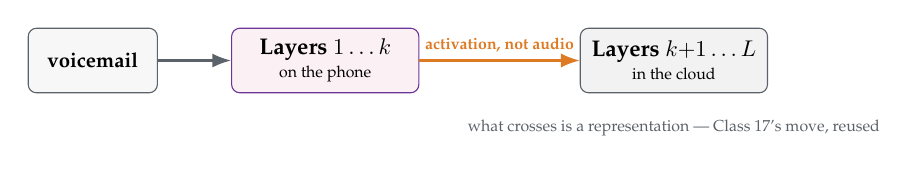
\begin{tikzpicture}[scale=0.82,transform shape]
    \node[endnode,minimum width=2.0cm] (in) at (0,0) {voicemail};
    \node[nnnode,minimum width=2.9cm,minimum height=1.0cm] (dev) at (3.6,0)
      {Layers $1 \ldots k$\\[-2pt]{\scriptsize\mdseries on the phone}};
    \node[chnode,minimum width=2.9cm,minimum height=1.0cm] (cl) at (9.0,0)
      {Layers $k{+}1 \ldots L$\\[-2pt]{\scriptsize\mdseries in the cloud}};
    \draw[flow] (in) -- (dev);
    \draw[flow,draw=coreorange,thick] (dev) -- node[iface,above]
      {activation, not audio} (cl);
    \node[lbl,visible on=<2->] at (9.0,-1.05)
      {what crosses is a representation --- Class 17's move, reused};
  \end{tikzpicture}

  \vspace{0.8em}
  \takeawayat{3-}{The raw data never leaves; the network carries an
    embedding.\\ Split point $k$ is a dial, not a fact.}
\end{frame}

% Teaching note (90 s): when splitting wins and when it embarrasses you. Wins: the
% early layers are cheap enough for the device, the activation is small, privacy or
% policy forbids shipping raw data. Loses: (1) if the activation is BIGGER than the
% input -- common for text prompts, where the input is a few KB and a single
% layer's hidden states are larger -- then just send the input; (2) the network
% round trip returns -- the latency we fled in section 2 is back in the loop;
% (3) if the cloud is unreachable, the split model is headless. So split inference
% shines for big sensory inputs (audio, video, sensor streams) with small useful
% representations -- not for short text.
\begin{frame}{When the cut wins --- and when it doesn't}
  \vspace{0.6em}
  \raggedright
  \textbf{Wins when}\par
  \begin{itemize}\itemsep4pt
    \item the input is big and sensory (audio, video), the representation small
    \item raw data must not leave the device
  \end{itemize}

  \vspace{0.6em}
  \uncover<2->{\textbf{Loses when}\par
  \begin{itemize}\itemsep4pt
    \item the activation is \emph{bigger} than the input --- a text prompt is a
      few KB; hidden states aren't
    \item the round trip we fled is back in the loop
    \item the cloud is gone --- a split model is headless offline
  \end{itemize}\par}

  \vspace{0.6em}
  \takeawayat{3-}{Split big-sensory, small-representation jobs.\\
    Don't split a text chat.}
\end{frame}

% Teaching note (100 s): collaboration without cutting -- speculative decoding. The
% small on-device model is fast but mediocre; the big cloud model is slow (and far)
% but authoritative. Let the small one DRAFT a few tokens, and the big one VERIFY
% the whole draft in a single parallel pass -- cheap, because checking k given
% tokens is one prefill-like pass, not k decode steps. Accepted tokens stream out;
% the first rejected one is corrected and drafting resumes from there. Most drafts
% are accepted (easy words are easy), so the expensive model runs once per several
% tokens. Same trick works entirely on-device between a tiny and a mid model.
% This is "collaborative inference": both models, each where it is strongest.
\begin{frame}{Or collaborate: draft small, verify big}
  \vspace{0.6em}
  \centering
  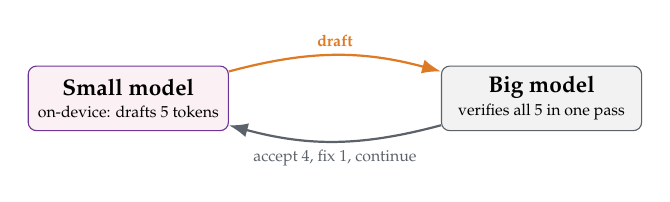
\begin{tikzpicture}[scale=0.82,transform shape]
    \node[nnnode,minimum width=3.1cm,minimum height=1.0cm] (s) at (0,0)
      {Small model\\[-2pt]{\scriptsize\mdseries on-device: drafts 5 tokens}};
    \node[chnode,minimum width=3.1cm,minimum height=1.0cm] (b) at (6.4,0)
      {Big model\\[-2pt]{\scriptsize\mdseries verifies all 5 in one pass}};
    \draw[flow,draw=coreorange,thick] (s) to[bend left=15]
      node[iface,above] {draft} (b);
    \draw[flow] (b) to[bend left=15] node[lbl,below]
      {accept 4, fix 1, continue} (s);
  \end{tikzpicture}

  \vspace{0.7em}
  \raggedright
  Checking $k$ given tokens is \textbf{one} parallel pass --- not $k$ slow
  decode steps. Easy words are easy: most drafts survive.\par

  \vspace{0.6em}
  \takeawayat{2-}{The big model runs once per \emph{several} tokens;\\
    the small one hides the distance. Speed without losing the big model's
    judgment.}
  \plainsource{Leviathan et al., ``Fast Inference from Transformers via
    Speculative Decoding,'' ICML 2023.}
\end{frame}

% Teaching note (60 s): one-frame summary of the section before routing. The
% boundary between the device and the cloud is a design dial with settings, not a
% wall: all-local (sections 3-5), cut at a layer, draft-and-verify, all-cloud.
% What's missing is the decision rule for choosing per request -- that is routing,
% the final trick.
\begin{frame}{The boundary is a dial}
  \vspace{0.8em}
  \centering
  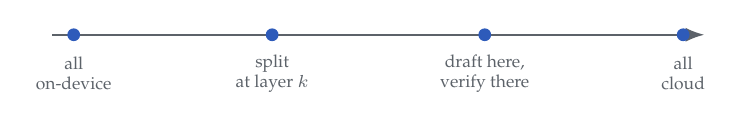
\begin{tikzpicture}[scale=0.9,transform shape]
    \draw[flow] (0,0) -- (9.2,0);
    \node[lbl,align=center] at (0.3,-0.55) {all\\on-device};
    \node[lbl,align=center] at (3.1,-0.55) {split\\at layer $k$};
    \node[lbl,align=center] at (6.1,-0.55) {draft here,\\verify there};
    \node[lbl,align=center] at (8.9,-0.55) {all\\cloud};
    \foreach \x in {0.3,3.1,6.1,8.9}{\fill[ranblue] (\x,0) circle (0.09);}
  \end{tikzpicture}

  \vspace{1.0em}
  \takeawayat{2-}{Four settings on one dial.\\
    Last question: \textbf{who turns the dial}, per request?}
\end{frame}

%!TEX root = ./main.tex

\section[Routing]{Model Routing}

% SECTION TIMING: 45:00--48:00 (3 frames): 70 + 70 + 40 s.

% Teaching note (70 s): the idea is almost social: a receptionist who answers the
% easy questions personally and forwards the hard ones to a specialist. Per query,
% a router sends easy requests to the local small model and hard ones to the cloud.
% Most requests are easy (set a timer, summarize a note), so the expensive path is
% exercised rarely -- the average cost drops while the worst-case quality is kept.
\begin{frame}{Trick 5: send the question, not every question}
  \vspace{0.7em}
  \centering
  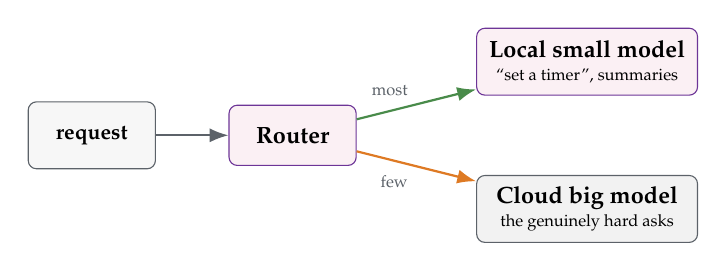
\begin{tikzpicture}[scale=0.85,transform shape]
    \node[endnode,minimum width=1.9cm] (q) at (0,0) {request};
    \node[nnnode,minimum width=1.9cm,minimum height=0.9cm] (r) at (3.0,0)
      {Router};
    \node[nnnode,minimum width=3.3cm,minimum height=1.0cm] (loc) at (7.4,1.1)
      {Local small model\\[-2pt]{\scriptsize\mdseries ``set a timer'',
        summaries}};
    \node[chnode,minimum width=3.3cm,minimum height=1.0cm] (cl) at (7.4,-1.1)
      {Cloud big model\\[-2pt]{\scriptsize\mdseries the genuinely hard asks}};
    \draw[flow] (q) -- (r);
    \draw[flow,draw=softgreen,thick] (r) -- node[lbl,above left] {most} (loc);
    \draw[flow,draw=coreorange] (r) -- node[lbl,below left] {few} (cl);
  \end{tikzpicture}

  \vspace{0.8em}
  \takeawayat{2-}{Average cost of the small model,\\
    worst-case quality of the big one.}
\end{frame}

% Teaching note (70 s): how does the router know a request is hard, before
% answering it? Three practical signals, cheapest first: (1) task type and length
% -- a timer is local by rule, a 30-page analysis is cloud by rule; (2) the small
% model's own confidence -- answer locally, and escalate when its token
% probabilities look unsure (students saw confidence in the PyTorch lecture);
% (3) a small learned router trained on pairs where people preferred the big
% model's answer. This is the shipped architecture: Apple's requests route between
% the ~3B on-device model and Private Cloud Compute; Pixel routes between Gemini
% Nano and the cloud Gemini.
\begin{frame}{How the router decides}
  \vspace{0.6em}
  \raggedright
  \begin{enumerate}[<+->]\itemsep6pt
    \item \textbf{Rules}: task type and length --- timers local,
      30-page analysis cloud
    \item \textbf{Confidence}: answer locally; escalate when the small model's
      own token probabilities look unsure
    \item \textbf{A learned router}: trained on requests where people preferred
      the big model's answer
  \end{enumerate}

  \vspace{0.7em}
  \uncover<4->{\raggedright This is the shipped design: Apple routes between its
    on-device model and Private Cloud Compute; Pixel between Gemini Nano and
    cloud Gemini.\par}
  \plainsource{Apple, ``Introducing Apple's On-Device and Server Foundation
    Models,'' 2024.}
\end{frame}

% Teaching note (40 s): close the five-trick arc with the complete picture: the
% modern assistant is not one model, it is a routed system of models -- quantized
% local ones, MoE cloud ones, caches and split points in between. Hand to wrap-up.
\begin{frame}{The assistant was never one model}
  \vspace{1.0em}
  \raggedright
  What answers you is a \textbf{system}: a router, a quantized on-device model,
  a KV cache on a diet, and an MoE in the cloud --- with split points and
  drafts in between.\par

  \vspace{1.0em}
  \takeawayat{2-}{``Where should the model run?'' ---\\
    the shipped answer is: \textbf{everywhere, each part where it is cheapest.}}
\end{frame}

%!TEX root = ./main.tex

\section[Wrap-up]{Wrap-Up}

% SECTION TIMING: 48:00--50:00 (3 frames): 60 + 40 + 20 s.

% Teaching note (60 s): the decision map, read as a flowchart in words. Start from
% the budget wall each question hits, and name the trick that answers it. This is
% the one slide to photograph.
\begin{frame}{One map of today}
  \vspace{0.5em}
  \centering
  \begin{tabular}{@{}ll@{}}
    \toprule
    \textbf{The wall} & \textbf{The trick}\\
    \midrule
    Weights don't fit & Quantization: fewer bits per weight\\
    Reading them is slow & Quantization again: fewer bytes per token\\
    Need more capacity & MoE: store big, read small\\
    Long chats eat RAM & KV cache: share, quantize, evict\\
    Still too big & Split: send the representation\\
    Cloud too slow/far & Collaborate: draft small, verify big\\
    Most queries are easy & Route: local first, escalate the hard\\
    \bottomrule
  \end{tabular}

  \vspace{0.8em}
  \takeawayat{2-}{One budget --- bytes in memory, bytes moved, joules ---\\
    and every trick is a way to spend less of it.}
\end{frame}

% Teaching note (40 s): what to remember, deliberately only three lines.
\begin{frame}{If you remember three things}
  \vspace{0.8em}
  \raggedright
  \begin{enumerate}\itemsep9pt
    \item On a phone, LLM decode is \textbf{bandwidth-bound}: tokens/s
      $\approx$ bandwidth $\div$ bytes per token
    \item Quantization, MoE, and the KV diet are all the \textbf{same move}:
      fewer bytes
    \item Device vs.\ cloud is a \textbf{dial} --- split, draft, route ---
      not a wall
  \end{enumerate}
\end{frame}

% Teaching note (20 s): logistics and handoff to Lex. HW4 due Wednesday 11/4;
% final project released 11/4; Wednesday's class: D2MoE (Paper Practicum).
\begin{frame}{Next}
  \vspace{0.9em}
  \raggedright
  \begin{itemize}\itemsep8pt
    \item \textbf{Now}: Lex presents \textbf{MobileMoE} (15 min + 5 min Q\&A)
    \item \textbf{Wednesday 11/4}: D2MoE --- experts that don't fit in memory
    \item HW4 due \textbf{11/4, 11:59 p.m.\ ET}; final project released 11/4
  \end{itemize}

  \vspace{1.2em}
  \centering
  {\large Questions?}
\end{frame}


\end{document}
